%=====================================================================
%  AI -> MACHINE LEARNING -> DATA SCIENCE
%  The cluster at a glance, Fall 2026
%
%  One A4 landscape page showing the three-course progression, the six
%  parts of each course, and -- the point of the page -- which course
%  OWNS each shared topic and which merely signposts or recaps it.
%
%  Deliberately self-contained: it does not \input any of the three
%  handouts or their .sty files, so it can be built and circulated on
%  its own. Palette and node styles are lifted from
%  "Data Science Fall 2026/DataScience_Fall2026_CourseAtAGlance.tex"
%  so the one-pagers read as one family.
%
%  Two layout notes, both learnt the hard way:
%   * The lane block's natural width is set close to the text width, so
%     \resizebox barely scales it. Scaling UP to \linewidth also scales
%     the height, and that is what pushes the page to two.
%   * \owns, \th, \sign and \nil are already defined by LaTeX or amssymb.
%     The chip macros here are \tOwn, \tSign, \tRecap, \tNil, \tHead.
%
%  Sources of record:
%    Artificial Intelligence Fall 2026/parts/G_schedule.tex
%    Machine Learning Fall 2026/README.md, parts/F_schedule.tex
%    Data Science Fall 2026/DataScience_Fall2026_CourseAtAGlance.tex
%    HEC AI-DS Curriculum Map/HEC_AI_DS_Curriculum_Map.tex
%
%  Build:  pdflatex -interaction=nonstopmode AI_ML_DS_Fall2026_ProgressionAtAGlance.tex
%=====================================================================
\documentclass[11pt]{article}
\usepackage[a4paper,landscape,top=0.8cm,bottom=0.7cm,left=1.1cm,right=1.1cm]{geometry}
\usepackage{lmodern}
\usepackage[T1]{fontenc}
\usepackage[utf8]{inputenc}
\usepackage[table]{xcolor}
\usepackage{graphicx}
\usepackage{array,ragged2e}
\usepackage{booktabs}
\usepackage{tikz}
\usetikzlibrary{arrows.meta,positioning}
\usepackage{fontawesome5}
\pagestyle{empty}
\setlength{\parindent}{0pt}

% Palette, lifted from the three handout style files
\definecolor{primary}{HTML}{1A5276}
\definecolor{secondary}{HTML}{2E86C1}
\definecolor{accent}{HTML}{C0392B}
\definecolor{greenhl}{HTML}{27AE60}
\definecolor{purplehl}{HTML}{8E44AD}
\definecolor{goldhl}{HTML}{B7950B}
\definecolor{tealhl}{HTML}{117A65}
\definecolor{lightbg}{HTML}{EBF5FB}
\definecolor{neutral}{HTML}{707B7C}
\definecolor{sub}{HTML}{465152}
% one hue per course, for the gutter and the ownership chips
\definecolor{aihue}{HTML}{1A5276}
\definecolor{mlhue}{HTML}{1E8449}
\definecolor{dshue}{HTML}{8A6D0A}

\newcolumntype{L}[1]{>{\RaggedRight\arraybackslash}p{#1}}

%--- ownership chips (names chosen to avoid LaTeX's own \owns, \th ...) -
\newcommand{\tOwn}[2]{{\setlength{\fboxsep}{1.8pt}\colorbox{#1}{%
  \fontsize{5.8}{6.8}\selectfont\bfseries\color{white}OWNS}}\
  {\fontsize{6.2}{7.2}\selectfont\bfseries\color{#1}#2}}
\newcommand{\tSign}[2]{{\setlength{\fboxsep}{1.4pt}\fcolorbox{#1}{white}{%
  \fontsize{5.8}{6.8}\selectfont\bfseries\color{#1}signpost}}\
  {\fontsize{6.2}{7.2}\selectfont\color{neutral}#2}}
\newcommand{\tRecap}[2]{{\setlength{\fboxsep}{1.4pt}\fcolorbox{#1}{white}{%
  \fontsize{5.8}{6.8}\selectfont\bfseries\color{#1}recap}}\
  {\fontsize{6.2}{7.2}\selectfont\color{neutral}#2}}
\newcommand{\tNil}{{\color{neutral!70}---}}
\newcommand{\tQ}[1]{\par{\fontsize{5.5}{6.3}\selectfont\itshape\color{neutral}#1}}
\newcommand{\tHead}[1]{{\bfseries\color{white}\fontsize{6.4}{7.4}\selectfont #1}}
\newcommand{\tCourse}[3]{\parbox[t]{1.7cm}{\raggedright
  {\fontsize{7.6}{8.6}\selectfont\bfseries\color{#1}#2}\\[0.5pt]
  {\fontsize{5.6}{6.4}\selectfont\color{neutral}Semester #3}}}

\begin{document}

%=====================================================================
% Title
%=====================================================================
\begin{center}
{\large\bfseries\color{aihue}ARTIFICIAL INTELLIGENCE}\ \
{\color{neutral}$\longrightarrow$}\ \
{\large\bfseries\color{mlhue}MACHINE LEARNING}\ \
{\color{neutral}$\longrightarrow$}\ \
{\large\bfseries\color{dshue}DATA SCIENCE}\\[2pt]
{\footnotesize\color{sub}The three-course progression at a glance\ \textbullet\
BSIT, Fall 2026\ \textbullet\ The Islamia University of Bahawalpur,
Department of Information Technology}\\[2pt]
{\color{secondary}\rule{\linewidth}{1.1pt}}
\end{center}

\vspace{-1pt}

%=====================================================================
% The three lanes: parts as chips, chapters compressed underneath.
% Natural width ~26.4cm against a text width of 27.5cm, so the
% resizebox scales by about 1.04 and the height is left alone.
%=====================================================================
\noindent\resizebox{\linewidth}{!}{%
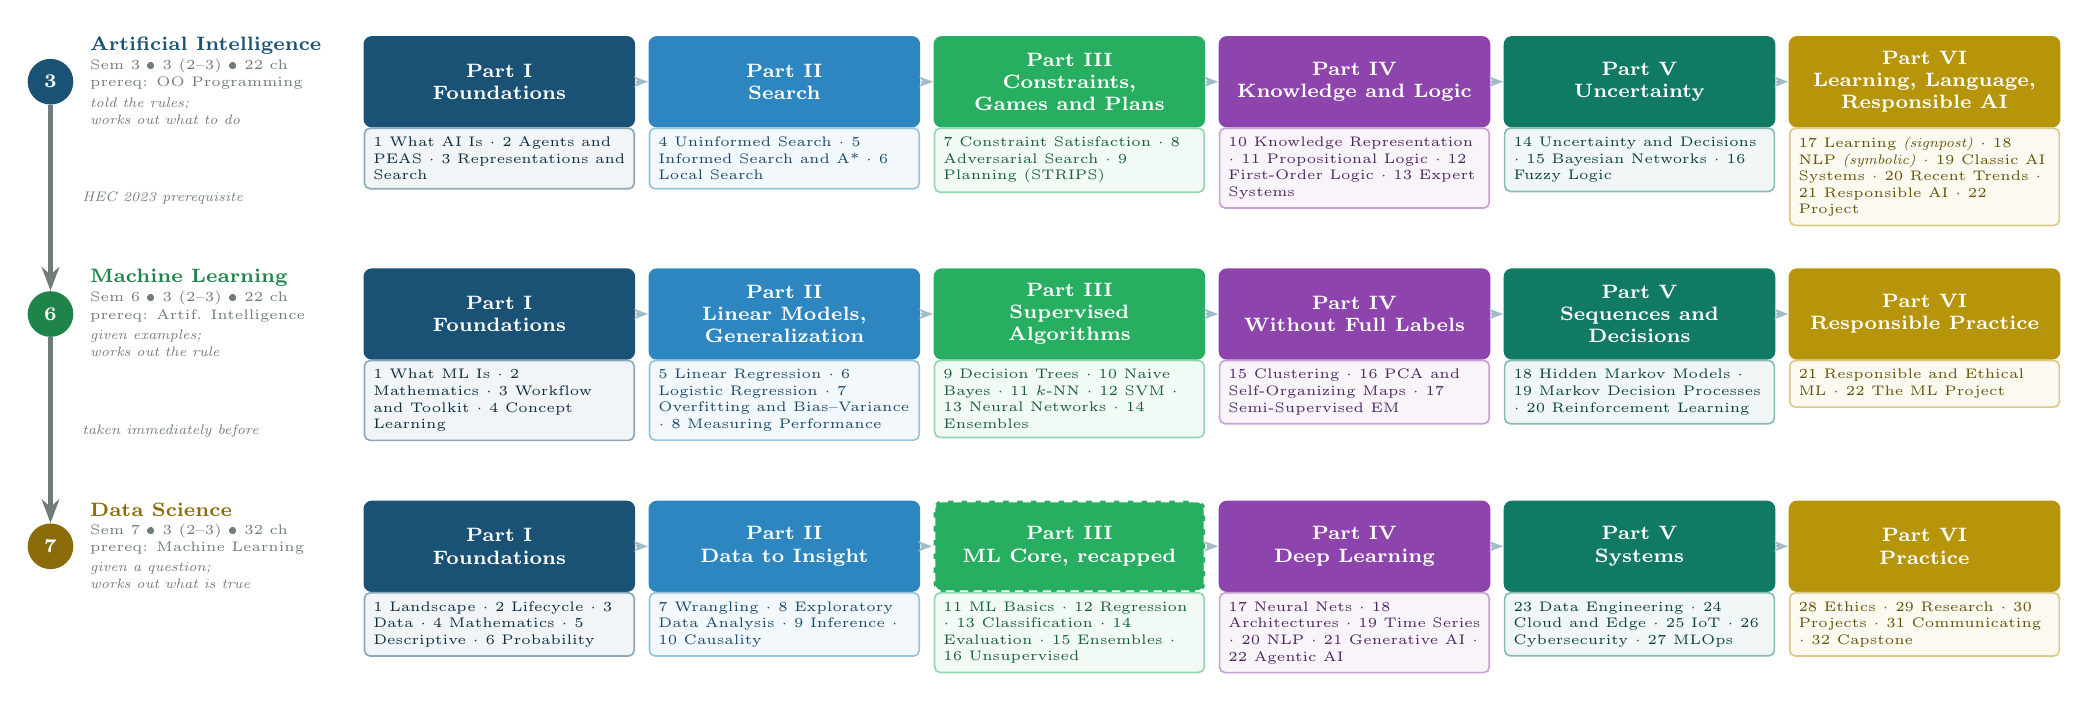
\begin{tikzpicture}[
  % text width lets a three-word part title wrap INSIDE the chip instead of
  % spilling over its neighbour; minimum width keeps the chips a uniform size.
  part/.style={rounded corners=3pt, fill=#1, text=white,
               font=\bfseries\scriptsize, minimum width=3.45cm,
               text width=3.05cm, minimum height=1.16cm, align=center,
               inner sep=2.5pt},
  chs/.style={rounded corners=2pt, draw=#1!50, line width=0.6pt, fill=#1!6,
              text=#1!55!black, font=\tiny, text width=3.2cm,
              align=flush left, inner sep=3.2pt, anchor=north},
  arr/.style={-{Stealth[length=1.8mm]}, primary!40, line width=0.7pt},
  preq/.style={-{Stealth[length=3mm]}, neutral, line width=1.5pt},
  cname/.style={font=\bfseries\scriptsize, text=#1, anchor=west},
  sem/.style={circle, fill=#1, text=white, font=\bfseries\scriptsize,
              minimum size=0.58cm, inner sep=0pt},
  meta/.style={font=\tiny, text=neutral, anchor=west}
]

%---------------------------------------------------------------------
% LANE 1 -- ARTIFICIAL INTELLIGENCE
%---------------------------------------------------------------------
\node[sem=aihue] (sai) at (0.30,0) {3};
\node[cname=aihue] at (0.68,0.46) {Artificial Intelligence};
\node[meta] at (0.68,0.20) {Sem 3 \textbullet\ 3 (2--3) \textbullet\ 22 ch};
\node[meta] at (0.68,-0.02) {prereq: OO Programming};
\node[meta] at (0.68,-0.28) {\itshape told the rules;};
\node[meta] at (0.68,-0.48) {\itshape works out what to do};

\node[part=primary]   (a1) at (6.00,0)  {Part I\\Foundations};
\node[part=secondary] (a2) at (9.62,0)  {Part II\\Search};
\node[part=greenhl]   (a3) at (13.24,0) {Part III\\Constraints,\\Games and Plans};
\node[part=purplehl]  (a4) at (16.86,0) {Part IV\\Knowledge and Logic};
\node[part=tealhl]    (a5) at (20.48,0) {Part V\\Uncertainty};
\node[part=goldhl]    (a6) at (24.10,0) {Part VI\\Learning, Language,\\Responsible AI};

\node[chs=primary]   at (6.00,-0.58)  {1 What AI Is $\cdot$ 2 Agents and PEAS $\cdot$ 3 Representations and Search};
\node[chs=secondary] at (9.62,-0.58)  {4 Uninformed Search $\cdot$ 5 Informed Search and A* $\cdot$ 6 Local Search};
\node[chs=greenhl]   at (13.24,-0.58) {7 Constraint Satisfaction $\cdot$ 8 Adversarial Search $\cdot$ 9 Planning (STRIPS)};
\node[chs=purplehl]  at (16.86,-0.58) {10 Knowledge Representation $\cdot$ 11 Propositional Logic $\cdot$ 12 First-Order Logic $\cdot$ 13 Expert Systems};
\node[chs=tealhl]    at (20.48,-0.58) {14 Uncertainty and Decisions $\cdot$ 15 Bayesian Networks $\cdot$ 16 Fuzzy Logic};
\node[chs=goldhl]    at (24.10,-0.58) {17 Learning \emph{(signpost)} $\cdot$ 18 NLP \emph{(symbolic)} $\cdot$ 19 Classic AI Systems $\cdot$ 20 Recent Trends $\cdot$ 21 Responsible AI $\cdot$ 22 Project};

\foreach \x/\y in {a1/a2,a2/a3,a3/a4,a4/a5,a5/a6}{\draw[arr] (\x) -- (\y);}

%---------------------------------------------------------------------
% LANE 2 -- MACHINE LEARNING
%---------------------------------------------------------------------
\node[sem=mlhue] (sml) at (0.30,-2.95) {6};
\node[cname=mlhue] at (0.68,-2.49) {Machine Learning};
\node[meta] at (0.68,-2.75) {Sem 6 \textbullet\ 3 (2--3) \textbullet\ 22 ch};
\node[meta] at (0.68,-2.97) {prereq: Artif. Intelligence};
\node[meta] at (0.68,-3.23) {\itshape given examples;};
\node[meta] at (0.68,-3.43) {\itshape works out the rule};

\node[part=primary]   (m1) at (6.00,-2.95)  {Part I\\Foundations};
\node[part=secondary] (m2) at (9.62,-2.95)  {Part II\\Linear Models,\\Generalization};
\node[part=greenhl]   (m3) at (13.24,-2.95) {Part III\\Supervised Algorithms};
\node[part=purplehl]  (m4) at (16.86,-2.95) {Part IV\\Without Full Labels};
\node[part=tealhl]    (m5) at (20.48,-2.95) {Part V\\Sequences and\\Decisions};
\node[part=goldhl]    (m6) at (24.10,-2.95) {Part VI\\Responsible Practice};

\node[chs=primary]   at (6.00,-3.53)  {1 What ML Is $\cdot$ 2 Mathematics $\cdot$ 3 Workflow and Toolkit $\cdot$ 4 Concept Learning};
\node[chs=secondary] at (9.62,-3.53)  {5 Linear Regression $\cdot$ 6 Logistic Regression $\cdot$ 7 Overfitting and Bias--Variance $\cdot$ 8 Measuring Performance};
\node[chs=greenhl]   at (13.24,-3.53) {9 Decision Trees $\cdot$ 10 Naive Bayes $\cdot$ 11 $k$-NN $\cdot$ 12 SVM $\cdot$ 13 Neural Networks $\cdot$ 14 Ensembles};
\node[chs=purplehl]  at (16.86,-3.53) {15 Clustering $\cdot$ 16 PCA and Self-Organizing Maps $\cdot$ 17 Semi-Supervised EM};
\node[chs=tealhl]    at (20.48,-3.53) {18 Hidden Markov Models $\cdot$ 19 Markov Decision Processes $\cdot$ 20 Reinforcement Learning};
\node[chs=goldhl]    at (24.10,-3.53) {21 Responsible and Ethical ML $\cdot$ 22 The ML Project};

\foreach \x/\y in {m1/m2,m2/m3,m3/m4,m4/m5,m5/m6}{\draw[arr] (\x) -- (\y);}

%---------------------------------------------------------------------
% LANE 3 -- DATA SCIENCE
%---------------------------------------------------------------------
\node[sem=dshue] (sds) at (0.30,-5.90) {7};
\node[cname=dshue] at (0.68,-5.44) {Data Science};
\node[meta] at (0.68,-5.70) {Sem 7 \textbullet\ 3 (2--3) \textbullet\ 32 ch};
\node[meta] at (0.68,-5.92) {prereq: Machine Learning};
\node[meta] at (0.68,-6.18) {\itshape given a question;};
\node[meta] at (0.68,-6.38) {\itshape works out what is true};

\node[part=primary]   (d1) at (6.00,-5.90)  {Part I\\Foundations};
\node[part=secondary] (d2) at (9.62,-5.90)  {Part II\\Data to Insight};
\node[part=greenhl, draw=white, line width=1.2pt,
      dash pattern=on 3pt off 2pt]
                      (d3) at (13.24,-5.90) {Part III\\ML Core, recapped};
\node[part=purplehl]  (d4) at (16.86,-5.90) {Part IV\\Deep Learning};
\node[part=tealhl]    (d5) at (20.48,-5.90) {Part V\\Systems};
\node[part=goldhl]    (d6) at (24.10,-5.90) {Part VI\\Practice};

\node[chs=primary]   at (6.00,-6.48)  {1 Landscape $\cdot$ 2 Lifecycle $\cdot$ 3 Data $\cdot$ 4 Mathematics $\cdot$ 5 Descriptive $\cdot$ 6 Probability};
\node[chs=secondary] at (9.62,-6.48)  {7 Wrangling $\cdot$ 8 Exploratory Data Analysis $\cdot$ 9 Inference $\cdot$ 10 Causality};
\node[chs=greenhl]   at (13.24,-6.48) {11 ML Basics $\cdot$ 12 Regression $\cdot$ 13 Classification $\cdot$ 14 Evaluation $\cdot$ 15 Ensembles $\cdot$ 16 Unsupervised};
\node[chs=purplehl]  at (16.86,-6.48) {17 Neural Nets $\cdot$ 18 Architectures $\cdot$ 19 Time Series $\cdot$ 20 NLP $\cdot$ 21 Generative AI $\cdot$ 22 Agentic AI};
\node[chs=tealhl]    at (20.48,-6.48) {23 Data Engineering $\cdot$ 24 Cloud and Edge $\cdot$ 25 IoT $\cdot$ 26 Cybersecurity $\cdot$ 27 MLOps};
\node[chs=goldhl]    at (24.10,-6.48) {28 Ethics $\cdot$ 29 Research $\cdot$ 30 Projects $\cdot$ 31 Communicating $\cdot$ 32 Capstone};

\foreach \x/\y in {d1/d2,d2/d3,d3/d4,d4/d5,d5/d6}{\draw[arr] (\x) -- (\y);}

%---------------------------------------------------------------------
% prerequisite arrows -- down the gutter only, so they cross nothing
%---------------------------------------------------------------------
\draw[preq] (sai) -- (sml);
\node[font=\tiny\itshape, text=neutral, anchor=west] at (0.58,-1.48)
  {HEC 2023 prerequisite};
\draw[preq] (sml) -- (sds);
\node[font=\tiny\itshape, text=neutral, anchor=west] at (0.58,-4.43)
  {taken immediately before};

\end{tikzpicture}}

\vspace{3pt}

%=====================================================================
% The ownership table -- real type, outside the resizebox
%=====================================================================
{\fontsize{6.6}{7.8}\selectfont\bfseries\color{neutral}%
\MakeUppercase{Who owns each shared topic}\quad
\mdseries\itshape \textbf{OWNS} taught here, with labs and assessment\ \textbullet\
\textbf{signpost} named and pointed at, deliberately not taught\ \textbullet\
\textbf{recap} assumed known and revised, not taught from zero}

\vspace{2pt}

\begingroup
\setlength{\tabcolsep}{2.6pt}
\renewcommand{\arraystretch}{1.2}
\arrayrulecolor{primary!20}
\noindent\begin{tabular}{@{}L{1.7cm}L{3.34cm}L{3.34cm}L{3.34cm}L{3.34cm}L{3.34cm}L{3.34cm}L{3.34cm}@{}}
\rowcolor{primary}
\tHead{Course} & \tHead{Search \& Agents} & \tHead{Neural Networks} &
\tHead{Natural Language} & \tHead{RL / MDP} & \tHead{Generative \& Agentic} &
\tHead{Bayesian Reasoning} & \tHead{Ethics \& Responsibility} \\
\rowcolor{aihue!7}
\tCourse{aihue}{AI}{3} &
\tOwn{aihue}{Ch 2, 4--9} &
\tSign{aihue}{Ch 17: the perceptron and the XOR limit} &
\tOwn{aihue}{Ch 18, the \emph{symbolic} half: grammars, parsing, Eliza} &
\tSign{aihue}{Ch 17: one agent--reward figure} &
\tSign{aihue}{Ch 20: named as a trend} &
\tOwn{aihue}{Ch 15, \emph{inference} in a given network} &
\tOwn{aihue}{Ch 21}\tQ{can its reasoning be trusted and audited?} \\
\rowcolor{mlhue!7}
\tCourse{mlhue}{ML}{6} &
\tNil &
\tOwn{mlhue}{Ch 13, perceptron to backpropagation} &
\tNil &
\tOwn{mlhue}{Ch 18--20, HMMs, MDPs, Q-learning} &
\tNil &
\tOwn{mlhue}{Ch 10, \emph{learning} the parameters} &
\tOwn{mlhue}{Ch 21}\tQ{is the learned model fair?} \\
\rowcolor{dshue!7}
\tCourse{dshue}{DS}{7} &
\tNil &
\tRecap{dshue}{Ch 17--18, architectures at scale} &
\tOwn{dshue}{Ch 20, the \emph{neural} half: embeddings, transformers} &
\tNil &
\tOwn{dshue}{Ch 21--22, generative and agentic systems} &
\tOwn{dshue}{Ch 6, \emph{description}: distributions and priors} &
\tOwn{dshue}{Ch 28}\tQ{privacy, security, duty to the subject} \\
\bottomrule
\end{tabular}
\endgroup

\vspace{3pt}

%=====================================================================
% Footer
%=====================================================================
{\fontsize{6.3}{7.6}\selectfont\itshape\color{gray!72!black}%
\textbf{The distinction is not the technique --- it is where the rules come from.}
\emph{Artificial Intelligence} is \emph{told} the rules and must work out what to do,
so it can hand you a plan, a proof or an inference chain; it is deliberately symbolic
and stops at the perceptron. \emph{Machine Learning} is given examples and must work
out the rule, so it hands you a model and an error estimate. \emph{Data Science} is
given a question and messy data and must work out what is true, so it hands you a
decision and a caveat.
\textbf{Why AI teaches no machine learning:} Chapter 17 covers the three learning
paradigms the HEC 2017 outline names, works the perceptron numerically, shows why one
perceptron cannot represent exclusive-or, and hands over --- a signpost, not a unit.
Appendix F of the AI handout states each boundary chapter by chapter, including the
fourth, with \textbf{Knowledge Representation \& Reasoning} (HEC 2023, 3 (3-0),
prerequisite Artificial Intelligence), which takes description logic, ontology
languages, commonsense reasoning and explainable AI further than AI Chapters 10--16
do. \textbf{Part III of Data Science is dashed} because it belongs to Machine
Learning: those six chapters are recapped rather than taught from zero, and only
feature engineering and anomaly detection are genuinely new. Curriculum basis: the HEC
2017 and HEC 2023 published outlines and the HEC 2025 course learning outcomes, as
collected in \texttt{HEC AI-DS Curriculum Map/}.\par}

\end{document}
